\documentclass[11pt]{article}
\usepackage[a4paper,margin=22mm]{geometry}
\usepackage{amsmath,amssymb,bm,graphicx,booktabs,placeins}
\usepackage[T1]{fontenc}
\usepackage{newtxtext,newtxmath,microtype}
\usepackage[colorlinks=true,linkcolor=blue,urlcolor=blue]{hyperref}
\graphicspath{{../figures/reference/supplemental/}}
\renewcommand{\thefigure}{S\arabic{figure}}
\renewcommand{\thetable}{S\arabic{table}}
\renewcommand{\theequation}{S\arabic{equation}}
\renewcommand{\thesection}{\Roman{section}}
\renewcommand{\thesubsection}{\Alph{subsection}}
\setlength{\parindent}{1.2em}
\setlength{\parskip}{0.25em}
\setlength{\textfloatsep}{12pt}
\begin{document}
\begin{center}
{\Large\bfseries Supplemental Material for\\[3pt]
Disorder-Restored Strong Connectivity in Degree-Limited Spatial Networks}\par
\vspace{8pt}
Jinhao Zhang$^{1,2}$, Jialin Meng$^{1,2,3,4,*}$, and Tianyu Wang$^{1,2,3,5,*}$\par
\vspace{6pt}
{\small
$^1$School of Integrated Circuits, Shandong University, Shandong Key Laboratory of Next-Generation Semiconductor Technology and Systems, Jinan 250100, China\\
$^2$Suzhou Research Institute of Shandong University, Suzhou 215123, China\\
$^3$National International Innovation Center, Shanghai 201203, China\\
$^4$Key Laboratory of Computational Neuroscience and Brain-Inspired Intelligence (Fudan University), Ministry of Education, Shanghai 200433, P. R. China\\
$^5$State Key Laboratory of Crystal Materials, Shandong University, Jinan 250100, China\\[4pt]
$^*$Correspondence: \href{mailto:jlmeng@sdu.edu.cn}{jlmeng@sdu.edu.cn} and \href{mailto:tywang@sdu.edu.cn}{tywang@sdu.edu.cn}}
\end{center}
This supplement describes the numerical ensembles, parameter controls, spatial-intervention sensitivity, finite-size geometry, and boundary-deletion statistics supporting the Letter. Source tables and scripts are available in the \href{https://github.com/neuromorphicscience-sys/janus-disorder-connectivity}{public reproducibility repository}. All quantities use the graph and orientation definitions of the Letter. Literature references are provided in its reference list.
\section{Numerical ensembles and reproducibility}
\subsection{Graph construction and sample inventory}
All ensembles use independent uniform point positions in an open square $[0,L]^2$, with $N=\operatorname{round}(\sigma L^2)$. A source $i$ considers distinct vertices within $a=2R$ and retains up to $q$ targets with the largest projection on $\bm e_i=(\sin\theta_i,-\cos\theta_i)$. Geometry determines the candidate counts, and hence the source outdegrees. Orientations determine which candidates are selected. Projection ties have probability zero for the continuous distributions used here; the implementation uses vertex indices to resolve numerical ties reproducibly. The graph has no self-loops. We measure the largest strongly connected component (SCC) fraction $S=|C_{\max}|/N$, with a singleton giving $S=1/N$ when all components are trivial.

Unless stated otherwise, $q=7$ and $\sigma R^2=24$, and lengths are reported in units of $R$. The Gaussian ensemble draws $\theta_i=Wz_i$ modulo $2\pi$, with independent standard normal $z_i$. Positions and orientation values are sampled once for each realization and remain quenched during graph construction and analysis. Statistical summaries use the realization as the unit of observation. Median curves join sampled condition medians, and bands or bars denote their interquartile ranges (IQRs).

The analyses use overlapping archived cohorts. Their counts describe each analysis separately, rather than independent additions to a total sample size. The broad parameter inventory contains 29,148 distinct graph hashes at the listed sizes and connection budgets. The full-Gaussian finite-size summary combines 4,634 distinct graphs at $L/R=64,128,256,512$ and $0\leq W\leq0.90$. The filtered mass and geometry study contains 784 graphs at seven values $W=0.7975,0.805,0.815,0.84,0.86,0.88,0.90$. The internal-recurrence study contains 1,528 graphs at 24 values of $W$ in $[0.75,0.90]$, with 8--96 realizations per condition. The clean feedback-count benchmark uses 24 graphs at $W=0$.

The spatial intervention uses 16 frozen bases at each $W=0.79,0.80,0.81$, for 48 matched pairs. Its correlation-length extension uses the same 48 bases at each of four lengths. The boundary-deletion ensemble includes all available eligible $L/R=128$ Gaussian graphs at the four selected conditions: 96 at $W=0.805$, 48 at $0.815$, and 24 each at $0.86$ and $0.90$. Each is analyzed at three deletion widths. Exact condition counts and graph identities accompany the source tables.

\subsection{Frozen identities and deterministic replay}
The supplied manifests identify each frozen graph by its geometry and orientation seeds, parameters, and SHA-256 digest of the canonical compressed sparse row (CSR) structure. Graph construction stores target indices in sorted order. The digest concatenates the row pointer and column-index bytes of this representation. Before either intervention or deletion analysis, the original graph is reconstructed from its archived seeds and its digest is compared with the manifest. Replay refers to reconstruction of the existing realization, with the same points and orientation values.

All 48 intervention bases and all 192 deletion bases pass this replay comparison. At $\ell=4R$, both the reassigned graph digest and its SCC fraction reproduce the original 48-pair archive. Available feedback-label archives are checked by their file digests. For 24 additional frozen high-disorder graphs without retained label arrays, the sparse classifier is reapplied to the complete graph and its full-graph $S_1,S_2$ values agree with their archived values. The labels are then held fixed for all deletion widths.

The public repository supplies graph-level source tables, frozen seed manifests for these replays, the sparse classifier, analysis scripts, tests, and scripts for Figs.~S1--S8. Large transient graph arrays are unnecessary for reproducing the figures from the source tables. Reconstructing the deletion or intervention graphs from their manifests is a separate computation. The sample inventory is deduplicated by graph hash wherever archived campaigns overlap.

\FloatBarrier
\section{Robustness of disorder-restored connectivity}
\subsection{Connection-budget dependence}
Figure~\ref{fig:q} collects the archived Gaussian scans for $q=4,5,6,7,8,10,12$ at $L/R=128$. Increasing orientational disorder produces a large SCC in every listed scan, while the location and width of the finite-size restoration window depend on $q$. The sampled windows differ among budgets, so each panel displays its own measured range. Table~\ref{tab:coverage} gives all available sizes, control ranges, and realization counts used for these comparisons. The graph-level source table retains every sampled condition.

At $L/R=128$, the largest sampled condition medians range from $0.961$ at $q=4$ to $0.997$ at $q=10$. These observations establish restoration across the tested connection budgets. The scans provide finite-system comparisons of the same projection-ranked rule at high density.

\begin{table}[htbp]
\centering\small
\caption{Archived robustness coverage at $\sigma R^2=24$. The control range is the union over the listed sizes, rather than a common grid at every size. $n_{\rm cond}$ is the range of realization counts per sampled condition. Non-Gaussian and correlated rows use $q=7$. Numeric rank-field lengths denote the actual Gaussian covariance scales $(\ell_x,\ell_y)$ used by the generating kernel. Per-size coverage is supplied in the source tables.}\label{tab:coverage}
\begin{tabular}{llllrr}
\toprule
Ensemble & $L/R$ & Control & Sampled range & $n_{
m total}$ & $n_{
m cond}$ \\
\midrule
Gaussian, $q=4$ & 64,128,256 & $W$ & 0.89853--0.94902 & 2224 & 8--48 \\
Gaussian, $q=5$ & 64,128 & $W$ & 0.82--0.98 & 560 & 12--32 \\
Gaussian, $q=6$ & 64,128,256 & $W$ & 0.79--0.87 & 1060 & 12--48 \\
Gaussian, $q=7$ & 64,128,256,512 & $W$ & 0.75--0.9 & 4152 & 4--128 \\
Gaussian, $q=8$ & 64,128,256 & $W$ & 0.735--0.815 & 996 & 12--48 \\
Gaussian, $q=10$ & 64,128 & $W$ & 0.65--0.85 & 564 & 12--32 \\
Gaussian, $q=12$ & 64,128,256 & $W$ & 0.4--0.9 & 2768 & 8--48 \\
Bounded uniform & 64,128 & $A$ & 1.6--1.8 & 792 & 16--32 \\
von Mises & 64,128 & $\kappa$ & 2.1--2.9 & 1136 & 16--48 \\
Wrapped Laplace & 64,128 & $b$ & 0.3--1.1 & 2528 & 16--48 \\
Rank field, $(12,2)R$ & 64,128 & $\alpha$ & 0.036472--1 & 2344 & 16--48 \\
Rank field, $(2,12)R$ & 64,128 & $\alpha$ & 0--1 & 2376 & 16--48 \\
Rank field, $(2,2)R$ & 64,128 & $\alpha$ & 0.044613--1 & 2048 & 16--48 \\
Rank field, $(4,4)R$ & 64,128,256 & $\alpha$ & 0--0.45 & 1296 & 16--48 \\
Rank field, $(6,6)R$ & 64,128 & $\alpha$ & 0.063576--1 & 2312 & 16--48 \\
Rank field, $(12,12)R$ & 64,128 & $\alpha$ & 0.082958--1 & 1992 & 16--48 \\
\bottomrule
\end{tabular}
\end{table}

\begin{figure}[htbp]
\centering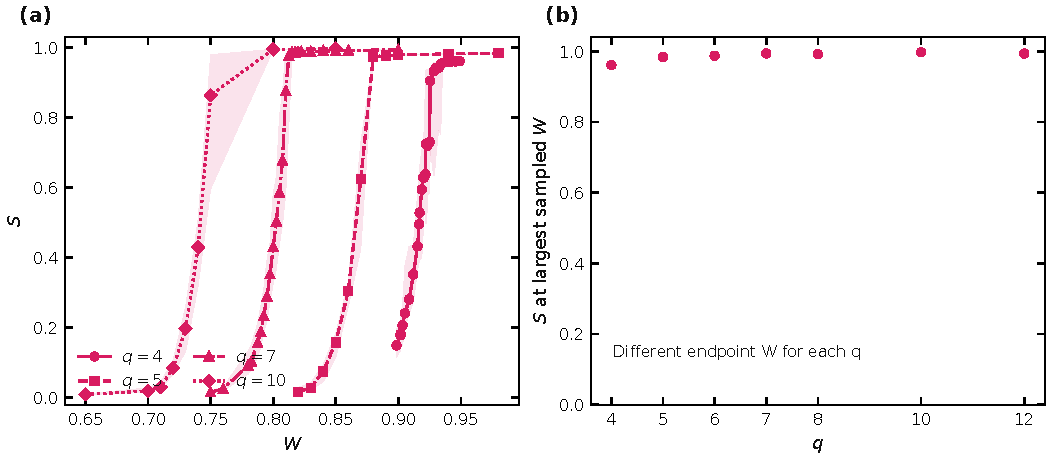
\includegraphics[width=\linewidth]{figS1.pdf}
\caption{Connection-budget robustness at $L/R=128$ and $\sigma R^2=24$: (a)--(g) $q=4,5,6,7,8,10,12$. Points and connecting lines show sampled condition medians, and bands show IQRs. Each panel uses the actual archived $W$ grid. The curves share the full-graph color and retain their separate disorder windows.}\label{fig:q}
\end{figure}

\subsection{Disorder families and spatial correlations}
The independent-mark controls use four distributions. Gaussian marks have standard deviation $W$ before wrapping. Bounded-uniform marks are sampled from $[-A,A]$. The von Mises density is $\exp(\kappa\cos\theta)/[2\pi I_0(\kappa)]$; smaller $\kappa$ gives broader directions. Wrapped-Laplace marks are obtained by wrapping a real Laplace variate of scale $b$. Figure~\ref{fig:families}(a)--(d) uses these native parameters on separate axes. Every family supports large strongly connected components over its measured range. Their numerical control values are distribution-specific.

The correlated controls retain a Gaussian orientation multiset at $W=0.82$. Its sorted values are assigned by the ranks of
\begin{equation}
 z_i(\alpha)=\sqrt{1-\alpha^2}\,\epsilon_i+\alpha\,\widetilde h(\bm r_i),\qquad 0\leq\alpha\leq1,
\end{equation}
where $\epsilon_i$ are independent normal variates and the sampled smooth field $\widetilde h$ is centered and normalized over the points. Gaussian smoothing of white noise uses widths $(\ell_x/\sqrt2,\ell_y/\sqrt2)$ on a grid of spacing $R$, followed by bilinear interpolation. Thus $\alpha=0$ is an independent permutation and $\alpha=1$ is a smooth spatial assignment. Intermediate $\alpha$ controls latent-field mixing.

Figure~\ref{fig:families}(e) displays isotropic covariance scales $\ell/R=2,4,6,12$; panel (f) displays anisotropic pairs $(\ell_x,\ell_y)/R=(12,2)$ and $(2,12)$. Increasing this smooth-field contribution changes connectivity even though the orientation multiset is preserved. These family scans report all archived outcomes and are distinct from the marginal-constrained intervention of Sec.~III.

Lengths in Fig.~\ref{fig:families} are taken from the smoothing parameters in the generating code. In particular, the historical data named ``2R'' used a smoothing width $4R/\sqrt2$ and therefore belong to the actual $\ell=4R$ family. The plotted numeric scale reflects that kernel. Both the earlier $256\times256$ canvas and its later $1024\times1024$ extension have margins exceeding the filter stencil around the observed crops, so periodic padding does not introduce wrapping through the sampled square. Table~\ref{tab:coverage} and the source tables preserve the actual lengths and native control parameters.

\begin{figure}[htbp]
\centering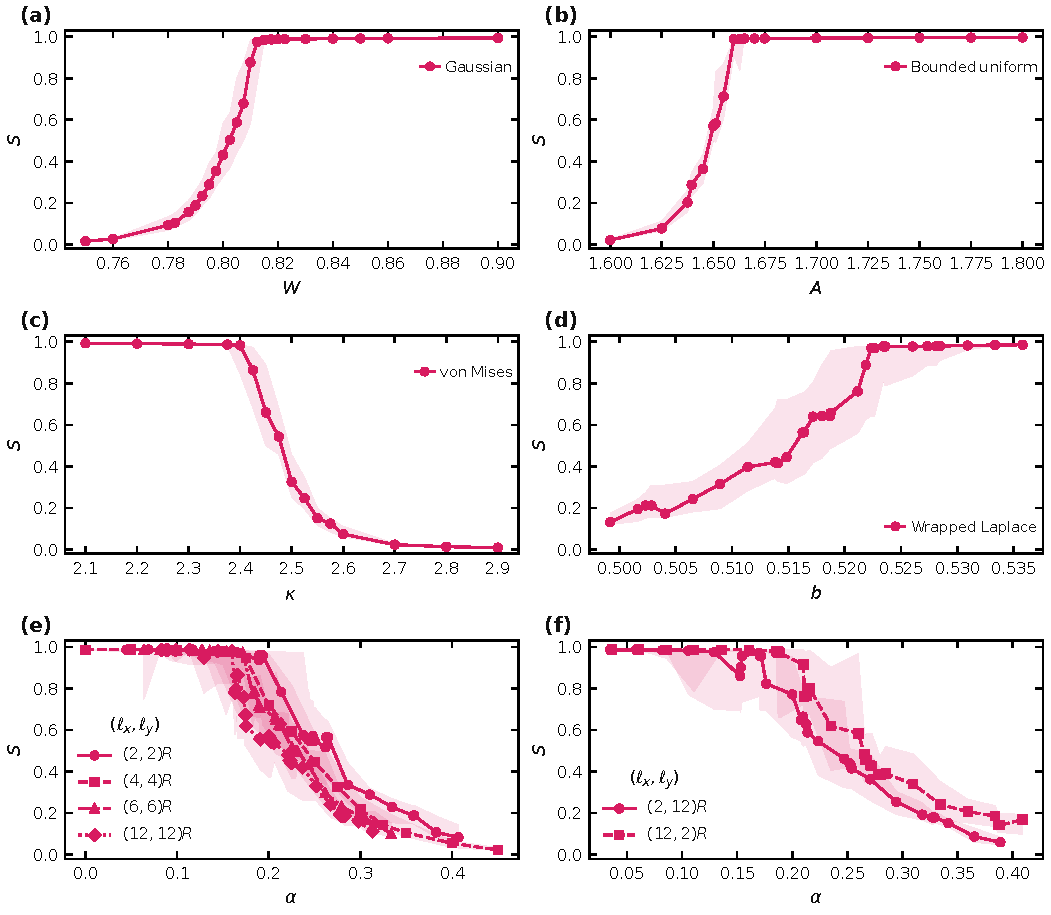
\includegraphics[width=\linewidth]{figS2.pdf}
\caption{Disorder-family and correlation controls at $q=7$, $L/R=128$, and $\sigma R^2=24$. (a) Gaussian standard deviation $W$. (b) Uniform half-width $A$. (c) von Mises concentration $\kappa$. (d) Laplace scale $b$. (e) Isotropic rank fields. (f) Anisotropic rank fields. Correlated scans retain a Gaussian multiset at $W=0.82$ and vary latent mixing $\alpha$. Curves are medians and bands are IQRs. Lines and markers distinguish the actual covariance scales in (e),(f).}\label{fig:families}
\end{figure}

\FloatBarrier
\section{Fixed-multiset spatial intervention}
\subsection{Full 48-pair fidelity statistics}
For a fixed point cloud and wrapped orientation multiset, the independent field is obtained from Gaussian noise on a $256\times256$ unit grid. The smoothed field is sampled at point coordinates shifted by $(64R,64R)$ with bilinear interpolation. Sorting these samples assigns the sorted orientations to the corresponding source ranks. This leaves positions, candidate counts, every outdegree, and the complete orientation multiset unchanged. The selected edges and indegrees may change.

The accepted intervention must preserve three measured full-edge marginals: edge length, wrapped angle relative to the source direction, and vertical displacement. For each marginal, the Kolmogorov--Smirnov distance and normalized Wasserstein distance must be at most $0.03$. The Wasserstein normalizers are $2R$, $\pi$, and $2R$, respectively. The empirical vertical-displacement rate is
\begin{equation}
 I_0=-\min_{0\leq t\leq32}\log\sum_b h_b e^{t x_b},
\end{equation}
using 2048 equal-width bins on $[-2R,2R]$, bin centers $x_b$, and normalized frequencies $h_b$. With $R$ as the numerical length unit, the relative rate change must satisfy
\begin{equation}
 \frac{|I_{0,r}-I_{0,o}|}{\max(I_{0,o},0.01)}\leq0.03.
\end{equation}
The changed-edge fraction must be at least $0.25$. A changed edge is an original source--target pair absent from the reassigned graph. All fidelity values are recorded before calculating the reassigned SCC fraction, and the same criteria apply to every correlation length.

Figure~\ref{fig:fidelity} displays all 48 original pairs at $\ell=4R$. The fidelity constraints accompany a strong connectivity reduction in every pair. Edge-length quantile changes use probabilities $0.10,0.25,0.50,0.75,0.90,0.95$ and are computed within each pair. The displacement CDF of the main figure pools edge counts; the fidelity distances here are assessed separately for each realization. This distinguishes pooled graphical agreement from pairwise acceptance.

At $\ell=4R$, the largest pairwise KS and normalized Wasserstein distances are $0.00395$ and $0.00141$, respectively. The largest relative $I_0$ change is $0.01646$, and the smallest changed-edge fraction is $0.74290$. These are maxima or minima across pairs, not averaged fidelity values.


\begin{figure}[htbp]
\centering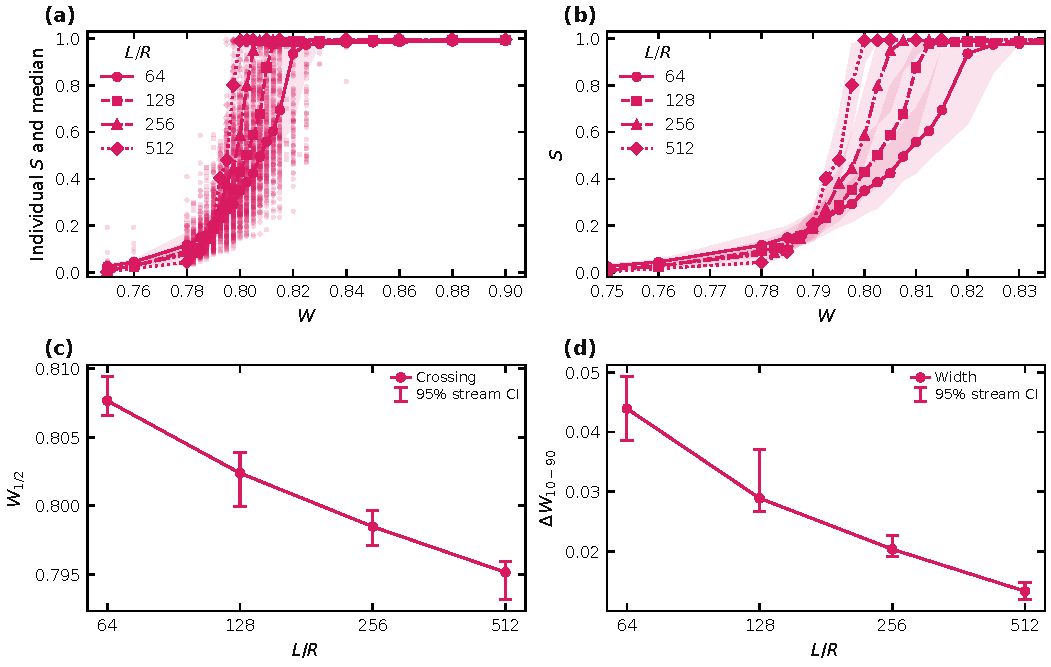
\includegraphics[width=\linewidth]{figS3.pdf}
\caption{All 48 canonical $\ell=4R$ intervention pairs. (a) Paired original and reassigned $S$. (b) Separate pairwise KS and normalized Wasserstein distances for the three marginals; the dashed line is $0.03$. (c) Paired edge-length quantile changes; points show individual pairs, and bars show IQRs about the median. (d) Connectivity suppression versus relative empirical-rate change. Every pair meets the common marginal constraints.}\label{fig:fidelity}
\end{figure}

\subsection{Correlation-length sensitivity}
The prespecified extension uses $\ell/R=1,2,4,8$ on the same 48 frozen bases. Each realization reuses the same underlying white-noise field across the four lengths; only the Gaussian smoothing width changes. The seed rule is also the historical rule for the canonical $\ell=4R$ pairs. There is one attempted reassignment per base and length, with no replacement of failed attempts.

Table~\ref{tab:ell} reports accepted counts and connectivity ratios. Figure~\ref{fig:ell}(a),(b) shows connectivity and local statistics for accepted pairs, whereas panels (c),(d) include all attempts. Local statistics are $A_{\rm loc}=\langle\cos\alpha\rangle$, $D=\langle-\Delta y/\ell_{ij}\rangle$, and $f_\uparrow=P(\Delta y>0)$ under the full-edge measure. Their changes accompany the complete pairwise marginal diagnostics.

\begin{table}[htbp]
\centering\small
\caption{Correlation-length sensitivity under the common fidelity criteria. Connectivity summaries use accepted pairs; rejected attempts remain in the supplied fidelity table. ``Max KS is the largest distance across all three marginals and accepted pairs, and ``Max rate change is the largest accepted relative change. The corresponding Wasserstein and changed-edge statistics appear in Fig.~
ef{fig:ell} and the source table.}\label{tab:ell}
\begin{tabular}{rrrcrrr}
\toprule
$\ell/R$ & Accepted & Rejected & Median $\log_{10}(S_r/S_o)$ & IQR & Max KS & Max rate change \\
\midrule
1 & 48/48 & 0 & -2.720 & [-2.957,-2.441] & 0.0022 & 0.0055 \\
2 & 48/48 & 0 & -3.267 & [-3.621,-3.084] & 0.0029 & 0.0116 \\
4 & 48/48 & 0 & -3.648 & [-3.840,-3.315] & 0.0040 & 0.0165 \\
8 & 42/48 & 6 & -3.718 & [-3.983,-3.447] & 0.0055 & 0.0133 \\
\bottomrule
\end{tabular}
\end{table}

The accepted median log ratios range from $-3.718$ to $-2.720$ across the four lengths. Every accepted reassignment suppresses connectivity. Thus the reduction persists over the accepted correlation scales with the same marginal criteria. Rejected attempts are retained as fidelity outcomes; their reassigned SCC fractions are not used in this comparison. The scale dependence concerns this fixed construction and sampled ensemble.


\begin{figure}[htbp]
\centering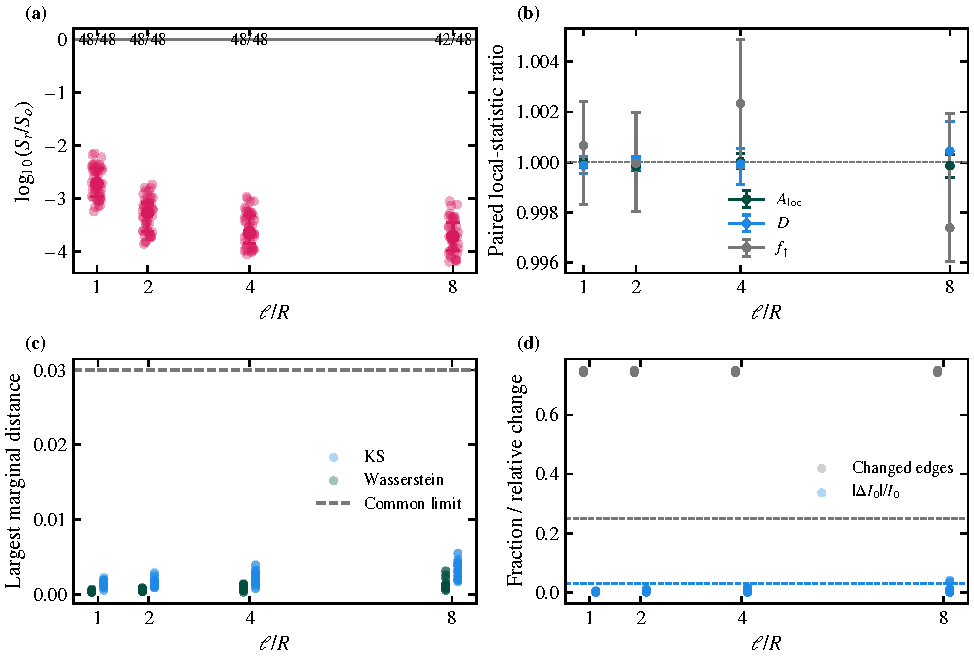
\includegraphics[width=\linewidth]{figS4.pdf}
\caption{Paired correlation-length sensitivity on 48 frozen bases at each $\ell/R$. (a) Individual accepted connectivity log ratios, median, and IQR; annotations give accepted/attempted counts. (b) Accepted local-statistic ratios, with IQRs. (c) Largest pairwise marginal KS and normalized Wasserstein distances, including rejected attempts. (d) Changed-edge fraction and relative rate change for all attempts. Dashed limits are $0.03$ for each distance and rate change, and $0.25$ as the minimum changed-edge fraction.}\label{fig:ell}
\end{figure}

\FloatBarrier
\section{Feedback-order filtration and finite-size geometry}
\subsection{Sparse classifier and structural invariants}
The strictly downward edges $D_0$ form a directed acyclic graph. Assign cost zero to those edges and cost one to upward feedback edges. For feedback edge $f=(u,v)$, the minimum return cost gives
\begin{equation}
 c(f)=1+\min_{P:v\rightsquigarrow u}\sum_{e\in P}\mathbf1_{e\in F}.
\end{equation}
Order one requires a downward return path from $v$ to $u$. An order-two witness consists of a distinct feedback edge $g=(s,t)$ and downward paths $v\rightsquigarrow s$ and $t\rightsquigarrow u$. Zero-length downward paths are included. Testing these witnesses determines the first two filtered graphs exactly.

The implementation makes forward and reverse searches on the downward DAG. Endpoint buckets identify candidate partner feedback edges. Geometric slabs shorten the searches without excluding a valid witness: if the maximum positive vertical edge displacement is $b$, a partner target satisfies $y_t\leq y_v+b$, and a partner source satisfies $y_s\geq y_u-b$. The algorithm stores sparse adjacency arrays and linear-size visit markers, rather than pairwise feedback reachability or a transitive closure. The retained graph is $G_k=D_0\cup\{f:c(f)\leq k\}$; a collective cycle assembled from its edges can contain more than $k$ feedback edges.

Classifier validation compares edge labels with independent bounded feedback-cost searches and small-graph downward reachability oracles. The archived checks include five synthetic graphs and 40 induced graphs from five frozen historical parents. They verify labels, return witnesses, SCC containment, and $S_1\leq S_2\leq S$. The public tests additionally cover empty feedback sets and reciprocal witnesses. Every filtered SCC lies inside an SCC of the full graph because filtration removes edges.

The first two orders serve as structural probes of low-order recurrence. Their largest components are compared with the full GSCC, while participation and concentration characterize the entire recurrent population. The edge-order labels and component sizes are separate observables.

\subsection{Finite-size restoration and surface geometry}
For the full Gaussian graph, all eligible archived scans are combined with the filtered mass cohort and deduplicated by graph hash. The resulting finite-size table contains 2,040 graphs at $L/R=64$, 1,584 at 128, 706 at 256, and 304 at 512. Their respective disorder grids contain 22, 25, 17, and 17 values. Figure~\ref{fig:finite} shows medians, IQRs, and sample variances. The source table also gives 95\% percentile bootstrap intervals for each median using 2,000 resamples of realizations within its condition.

For a level $p$, $W_p(L)$ is linearly interpolated only between adjacent sampled values whose medians bracket $p$. Table~\ref{tab:finite} reports $p=0.1,0.5,0.9$ and $\Delta W_{10-90}=W_{0.9}-W_{0.1}$. All listed levels have unique brackets in these four sampled curves. No values outside the sampled grid enter the interpolation. The source tables retain the two endpoints of every bracket.

\begin{table}[htbp]
\centering\small
\caption{Descriptive finite-size crossover diagnostics for Gaussian $q=7$, $\sigma R^2=24$. Crossing values are piecewise-linear interpolants of the median curve on its actual sampled grid.}\label{tab:finite}
\begin{tabular}{rrrrrrr}
\toprule
$L/R$ & $n$ & $n_W$ & $W_{0.1}$ & $W_{0.5}$ & $W_{0.9}$ & $\Delta W_{10-90}$ \\
\midrule
64 & 2040 & 22 & 0.775344 & 0.807662 & 0.819265 & 0.043921 \\
128 & 1584 & 25 & 0.781683 & 0.802383 & 0.810598 & 0.028915 \\
256 & 706 & 17 & 0.783824 & 0.798479 & 0.804215 & 0.020391 \\
512 & 304 & 17 & 0.785439 & 0.795150 & 0.798797 & 0.013358 \\
\bottomrule
\end{tabular}
\end{table}

The median half-height crossing shifts toward smaller $W$, from $0.807662$ to $0.795150$, while the 10--90\% width falls from $0.043921$ to $0.013358$. The crossover therefore drifts and sharpens over the investigated sizes. The sampled variance maxima also shift, but unequal disorder grids and sample counts limit their interpretation to sampled maxima. The descriptive crossings characterize these finite-size windows.

\begin{figure}[htbp]
\centering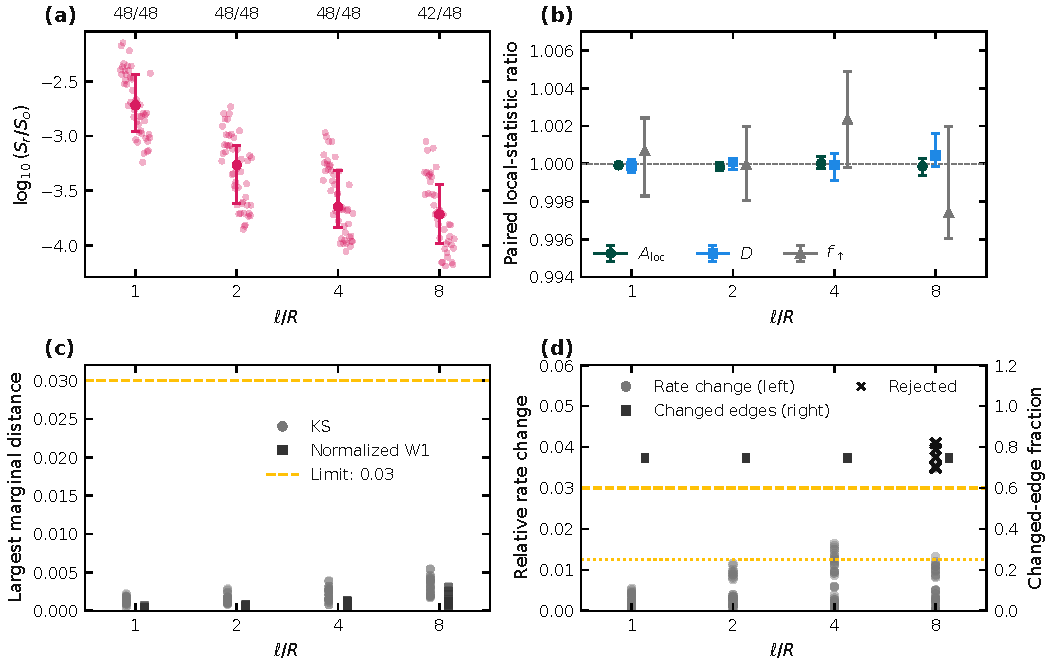
\includegraphics[width=\linewidth]{figS5.pdf}
\caption{Finite-size restoration diagnostics at Gaussian $q=7$, $\sigma R^2=24$. (a) Median $S(W)$ and IQR. (b) Sample variance of $S$. (c) Bracketed crossings $W_{0.1},W_{0.5},W_{0.9}$. (d) Interpolated 10--90\% width. Sizes use a common full-graph color with distinct markers and line styles in (a),(b). Straight segments interpolate sampled statistics. Variance points do not resolve a continuous peak.}\label{fig:finite}
\end{figure}

The separate 784-graph mass and geometry cohort measures the largest $G_1$ and $G_2$ components. At $W=0.7975,0.805,0.815$, $LS_k/R$ remains approximately size-independent across $L/R=64$--512 [Fig.~\ref{fig:geometry}(a),(b)]. At fixed density, this corresponds to largest-component mass of approximate order $L$ over the measured sizes. At $W=0.805$, the $G_2$ major span remains comparable to $L$, while its relative minor span decreases [panel (c)]. The typical largest components favor the downstream $2R$ strip [panel (d)].

Local occupancy $p_k(d)$ divides the number of largest-component members in a downstream-depth bin by all vertices in that bin. The penetration depth $d_{90}$ is the $\lceil0.9|C_{\max}|\rceil$th ordered depth within the component. The main figure compares these observables directly with the full GSCC. An $O(L)$ boundary extent with typical finite $O(R)$ penetration provides the geometric interpretation of this finite-size mass sector. It describes the largest low-order SCC, while other low-order SCCs occur throughout the interior.

Direction selection is tested by paired reversal and rotation on 24 frozen $L/R=128$, $W=0.805$ point clouds. Adding $\pi$ or $\pi/2$ to all angles changes the downstream side to top or right. The edges are reconstructed from the shifted directions, and classification uses the corresponding progress coordinate $-y$ or $-x$. Downstream-minus-opposite strip membership measures localization relative to that direction. For $G_2$, all original and rotated contrasts are positive; 22 reversed contrasts are positive and two are zero. This links the preferred surface to the directional field.

\begin{figure}[htbp]
\centering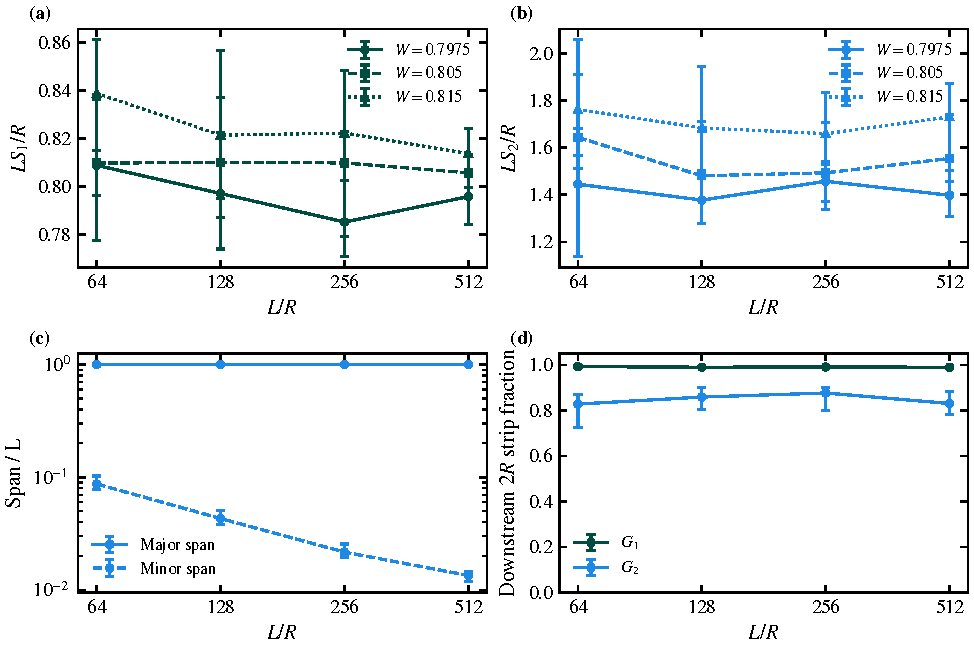
\includegraphics[width=\linewidth]{figS6.pdf}
\caption{Finite-size geometry of the largest low-order components. (a),(b) $LS_1/R$ and $LS_2/R$ at three near-restoration conditions; markers and line styles distinguish $W$. (c) Major and minor $G_2$ spans relative to $L$ at $W=0.805$. (d) Largest-component fraction in the downstream $2R$ strip at $W=0.805$. Points are condition medians and bars are IQRs. The finite-size mass cohort contains 784 graphs; panels use the indicated subsets.}\label{fig:geometry}
\end{figure}

\FloatBarrier
\section{Internal recurrence and boundary robustness}
\subsection{Internal recurrence in 1,528 realizations}
For the strict core
\begin{equation}
 I=\{i:4R<x_i<L-4R,\quad 4R<y_i<L-4R\},
\end{equation}
we restrict the classified graph to the induced subgraph $G_k[I]$. Nontrivial SCCs contain at least two vertices. If $M_k^{\rm int}$ counts vertices in all such SCCs and $C_k^{\rm int}$ is the largest, define
\begin{equation}
 f_{k,\rm rec}^{\rm int}=\frac{M_k^{\rm int}}{|I|},\qquad
 \eta_k^{\rm int}=\frac{|C_k^{\rm int}|}{M_k^{\rm int}}.
\end{equation}
Internal recurrent mass is nonzero in every analyzed graph, so the concentration ratio is defined throughout this ensemble. The graph-level identity $|C_k^{\rm int}|/|I|=f_{k,\rm rec}^{\rm int}\eta_k^{\rm int}$ separates participation from concentration. Products of their separate condition medians need not equal the median largest-component fraction.

At $W=0.815$, the full-graph median $S=0.985$ coexists with median internal $G_2$ participation $0.138$ and concentration $0.039$. Approximately $8.0\times10^3$ nontrivial internal components distribute that recurrent mass. At $W=0.90$, participation and concentration medians are $0.946$ and $0.996$. These are ensemble comparisons at distinct disorder values.

For a separate boundary-path check, parent recurrent mass counts core vertices that belong to nontrivial SCCs in the complete $G_k$. Internal mass requires paths to remain in the core. Their ratio in Fig.~\ref{fig:internal}(d) quantifies retention under this stronger path restriction. High retention near restoration shows that the internal recurrent population largely survives with its paths confined to the interior. The fragmented organization is also visible in the concentration and component-count statistics, rather than inferred solely from the small largest-component fraction.

\begin{figure}[htbp]
\centering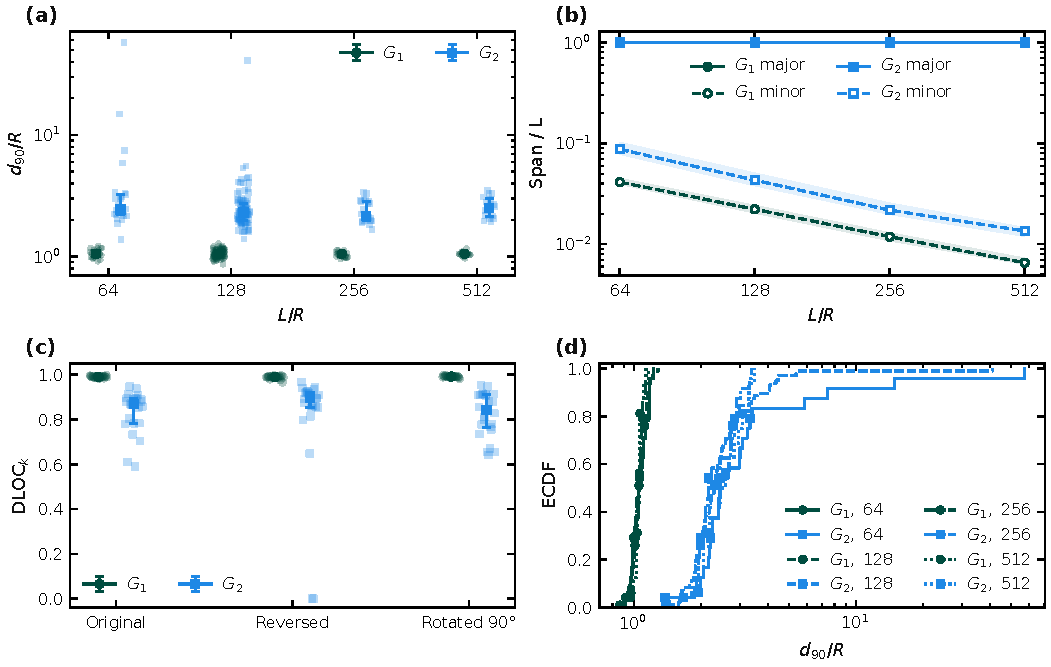
\includegraphics[width=\linewidth]{figS7.pdf}
\caption{Internal recurrence across 1,528 frozen Gaussian realizations at $L/R=128$, $q=7$. (a) Recurrent participation. (b) Largest-component concentration among recurrent vertices. (c) Number of nontrivial internal SCCs. (d) Internal/parent recurrent mass retention in the same core. Curves are medians and bands are IQRs; each sampled $W$ has 8--96 graphs. The gray region marks $0.7975\leq W\leq0.815$. Orders are classified in the complete graph.}\label{fig:internal}
\end{figure}

\subsection{Boundary-deletion ensemble and cut widths}
For deletion width $w$, the retained set is
\begin{equation}
 I_w=\{i:w<x_i<L-w,\quad w<y_i<L-w\}.
\end{equation}
We analyze $w/R=2,4,8$ on every eligible frozen graph at $W=0.805,0.815,0.86,0.90$. Edges are labeled in the complete graph first and then restricted to $I_w$; outgoing connections are not refilled. The reported fractions use $|I_w|$ as the denominator for the full and filtered graphs alike. The output table contains retained node counts, $S(G[I_w])$, $S(G_1[I_w])$, $S(G_2[I_w])$, their paired differences, and the full/$G_2$ ratio.

If orders are instead recomputed inside the core, the resulting hierarchy $H_k$ obeys $H_k\subseteq G_k[I_w]$: a return path in the induced graph was already available in the original graph, so deletion cannot lower its minimum feedback cost. The primary result uses the original labels and provides this upper bound on an internally relabeled hierarchy.

Table~\ref{tab:deletion} gives the complete paired distributions, and Fig.~\ref{fig:deletion} shows individual graphs at $4R$, width dependence, difference ECDFs, and the positions of the four main-figure representatives in the enlarged ensemble. Actual retained fractions are close to the geometric expectations $(1-2w/L)^2$, namely $0.9385,0.8789,0.7656$ at $L/R=128$.

\begin{table}[htbp]
\centering\small
\caption{All eligible frozen boundary-deletion graphs. Fractions are normalized by the retained core node count. The paired difference is $\Delta=S(G[I_w])-S(G_2[I_w])$; its median is computed from graph-level differences. Minima and maxima retain the full observed spread. The source tables give IQRs and $G_1$ values as well.}\label{tab:deletion}
\begin{tabular}{rrrrrrr}
\toprule
$W$ & $w/R$ & $n$ & Median full & Median $G_2$ & Median $\Delta$ & Range of $\Delta$ \\
\midrule
0.805 & 2 & 96 & 0.5671 & 0.0033 & 0.5641 & [0.2345,0.9557] \\
0.805 & 4 & 96 & 0.5512 & 0.0035 & 0.5483 & [0.2426,0.9537] \\
0.805 & 8 & 96 & 0.5382 & 0.0039 & 0.5345 & [0.2357,0.9500] \\
0.815 & 2 & 48 & 0.9488 & 0.0053 & 0.9420 & [0.4686,0.9570] \\
0.815 & 4 & 48 & 0.9405 & 0.0055 & 0.9292 & [0.4668,0.9541] \\
0.815 & 8 & 48 & 0.9397 & 0.0058 & 0.9306 & [0.3630,0.9532] \\
0.860 & 2 & 24 & 0.9663 & 0.1158 & 0.8487 & [0.7436,0.9343] \\
0.860 & 4 & 24 & 0.9659 & 0.1213 & 0.8446 & [0.7332,0.9330] \\
0.860 & 8 & 24 & 0.9622 & 0.1078 & 0.8554 & [0.7065,0.9223] \\
0.900 & 2 & 24 & 0.9703 & 0.9385 & 0.0308 & [0.0223,0.3325] \\
0.900 & 4 & 24 & 0.9697 & 0.9406 & 0.0295 & [0.0220,0.4080] \\
0.900 & 8 & 24 & 0.9673 & 0.9356 & 0.0312 & [0.0238,0.3653] \\
\bottomrule
\end{tabular}
\end{table}

The separation is strongest in the natural restoration window: full-graph interior connectivity is much larger than low-order interior connectivity at every deletion width, with realization-to-realization variation retained in the table. At high disorder, $G_2$ itself occupies much of the core, so the separation becomes smaller. The deletion result therefore distinguishes the near-restoration and high-disorder organizations of the filtered graph.

The four main-figure realizations were selected from the earlier mass-scaling cohort by minimizing the absolute deviation of full-graph $S_2$ from its condition median, with graph identifier as the tie-break. This selection preceded the present ensemble deletion calculation. It uses $S_2$ before deletion, rather than optimizing a core-connectivity difference. In order of increasing $W$, their realization identifiers are 70, 34, 14, and 6. The source table records their complete hashes and ensemble percentiles. Panel (d) locates them within the enlarged deletion ensemble. Their positions need not be central in every core statistic, which is why panels (a)--(c) retain all realizations.

The clean-limit boundary benchmark in the Letter evaluates the exact fixed-$N$ selection deficit before taking the high-density asymptote. The finite-$N$ prediction $907.006$ matches the 24-graph mean $906.75$; the sample standard deviation is $12.42$. The asymptotic value at the same finite $L$ is $906.816$. Feedback production in this clean source layer and recurrent component mass under disorder are distinct observables. The boundary calculation provides a microscopic benchmark for where clean feedback is generated, while the deletion ensembles test the organization of restored interior connectivity.

\begin{figure}[htbp]
\centering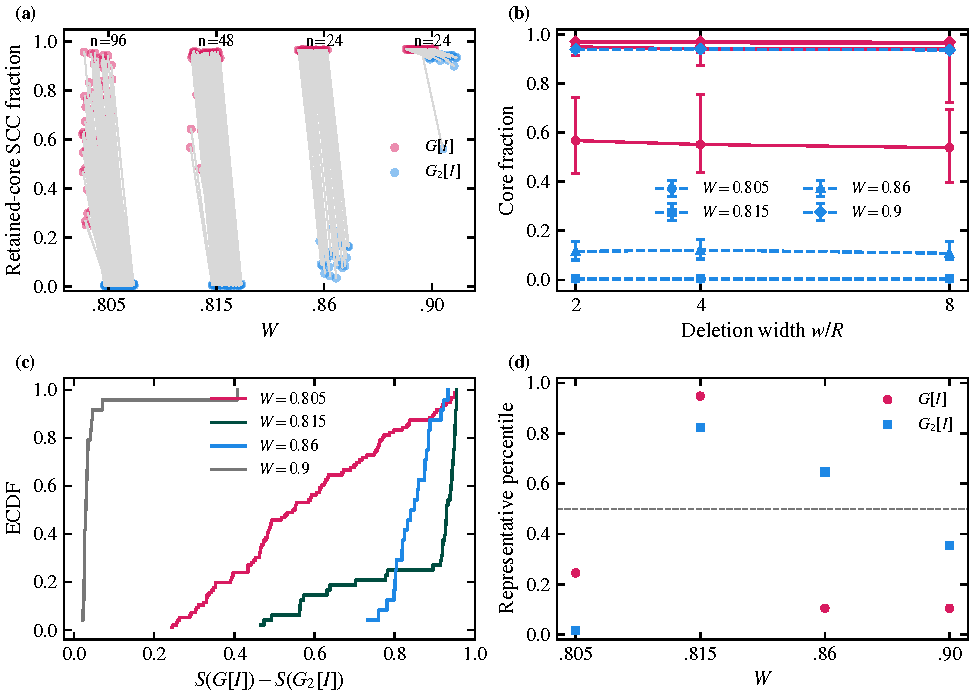
\includegraphics[width=\linewidth]{figS8.pdf}
\caption{Boundary deletion on all eligible $L/R=128$ frozen graphs. (a) Individual full and $G_2$ core fractions after $4R$ deletion, paired by faint connectors; counts are 96,48,24,24. (b) Medians and IQRs versus deletion width; full graph is magenta and $G_2$ is blue, while markers distinguish $W$. (c) ECDFs of paired full-minus-$G_2$ core fractions at $4R$. (d) Empirical percentiles of the four main-figure representatives within their corresponding $4R$ ensembles; ties receive midranks. Feedback labels are assigned before deletion.}\label{fig:deletion}
\end{figure}

\FloatBarrier
\end{document}
